% Options for packages loaded elsewhere
\PassOptionsToPackage{unicode}{hyperref}
\PassOptionsToPackage{hyphens}{url}
%
\documentclass[
  11pt,
]{article}
\usepackage{amsmath,amssymb}
\usepackage{lmodern}
\usepackage{iftex}
\ifPDFTeX
  \usepackage[T1]{fontenc}
  \usepackage[utf8]{inputenc}
  \usepackage{textcomp} % provide euro and other symbols
\else % if luatex or xetex
  \usepackage{unicode-math}
  \defaultfontfeatures{Scale=MatchLowercase}
  \defaultfontfeatures[\rmfamily]{Ligatures=TeX,Scale=1}
\fi
% Use upquote if available, for straight quotes in verbatim environments
\IfFileExists{upquote.sty}{\usepackage{upquote}}{}
\IfFileExists{microtype.sty}{% use microtype if available
  \usepackage[]{microtype}
  \UseMicrotypeSet[protrusion]{basicmath} % disable protrusion for tt fonts
}{}
\makeatletter
\@ifundefined{KOMAClassName}{% if non-KOMA class
  \IfFileExists{parskip.sty}{%
    \usepackage{parskip}
  }{% else
    \setlength{\parindent}{0pt}
    \setlength{\parskip}{6pt plus 2pt minus 1pt}}
}{% if KOMA class
  \KOMAoptions{parskip=half}}
\makeatother
\usepackage{xcolor}
\usepackage[margin=1.0in]{geometry}
\usepackage{graphicx}
\makeatletter
\def\maxwidth{\ifdim\Gin@nat@width>\linewidth\linewidth\else\Gin@nat@width\fi}
\def\maxheight{\ifdim\Gin@nat@height>\textheight\textheight\else\Gin@nat@height\fi}
\makeatother
% Scale images if necessary, so that they will not overflow the page
% margins by default, and it is still possible to overwrite the defaults
% using explicit options in \includegraphics[width, height, ...]{}
\setkeys{Gin}{width=\maxwidth,height=\maxheight,keepaspectratio}
% Set default figure placement to htbp
\makeatletter
\def\fps@figure{htbp}
\makeatother
\setlength{\emergencystretch}{3em} % prevent overfull lines
\providecommand{\tightlist}{%
  \setlength{\itemsep}{0pt}\setlength{\parskip}{0pt}}
\setcounter{secnumdepth}{5}
\newlength{\cslhangindent}
\setlength{\cslhangindent}{1.5em}
\newlength{\csllabelwidth}
\setlength{\csllabelwidth}{3em}
\newlength{\cslentryspacingunit} % times entry-spacing
\setlength{\cslentryspacingunit}{\parskip}
\newenvironment{CSLReferences}[2] % #1 hanging-ident, #2 entry spacing
 {% don't indent paragraphs
  \setlength{\parindent}{0pt}
  % turn on hanging indent if param 1 is 1
  \ifodd #1
  \let\oldpar\par
  \def\par{\hangindent=\cslhangindent\oldpar}
  \fi
  % set entry spacing
  \setlength{\parskip}{#2\cslentryspacingunit}
 }%
 {}
\usepackage{calc}
\newcommand{\CSLBlock}[1]{#1\hfill\break}
\newcommand{\CSLLeftMargin}[1]{\parbox[t]{\csllabelwidth}{#1}}
\newcommand{\CSLRightInline}[1]{\parbox[t]{\linewidth - \csllabelwidth}{#1}\break}
\newcommand{\CSLIndent}[1]{\hspace{\cslhangindent}#1}
\newcommand{\bcenter}{\begin{center}}
\newcommand{\ecenter}{\end{center}}
\newcommand{\btitlepage}{\begin{titlepage}}
\newcommand{\etitlepage}{\end{titlepage}}
\usepackage{setspace}\doublespacing
\usepackage{helvet}
\renewcommand*\familydefault{\sfdefault}
\usepackage{booktabs}
\usepackage[font=small,labelfont=bf]{caption}
\usepackage{booktabs}
\usepackage{longtable}
\usepackage{array}
\usepackage{multirow}
\usepackage{wrapfig}
\usepackage{float}
\usepackage{colortbl}
\usepackage{pdflscape}
\usepackage{tabu}
\usepackage{threeparttable}
\usepackage{threeparttablex}
\usepackage[normalem]{ulem}
\usepackage{makecell}
\usepackage{xcolor}
\ifLuaTeX
  \usepackage{selnolig}  % disable illegal ligatures
\fi
\IfFileExists{bookmark.sty}{\usepackage{bookmark}}{\usepackage{hyperref}}
\IfFileExists{xurl.sty}{\usepackage{xurl}}{} % add URL line breaks if available
\urlstyle{same} % disable monospaced font for URLs
\hypersetup{
  hidelinks,
  pdfcreator={LaTeX via pandoc}}

\author{}
\date{\vspace{-2.5em}}

\begin{document}

\begin{titlepage}

\begin{center}

\vspace*{30mm}

\hypertarget{an-agent-based-model-of-gender-differences-in-short-term-mating-behaviors-as-a-result-of-mating-preferences}{%
\section*{An Agent-Based Model of Gender Differences in Short-Term
Mating Behaviors as a Result of Mating
Preferences}\label{an-agent-based-model-of-gender-differences-in-short-term-mating-behaviors-as-a-result-of-mating-preferences}}
\addcontentsline{toc}{section}{An Agent-Based Model of Gender
Differences in Short-Term Mating Behaviors as a Result of Mating
Preferences}

\vspace{30mm}

Yurun Ying\textsuperscript{1}, Jan Antfolk\textsuperscript{2}, Pekka
Santtila\textsuperscript{1,3,\(\dagger\)}

\textsuperscript{1} Faculty of Arts and Sciences, NYU Shanghai

\textsuperscript{2} Faculty of Arts, Psychology and Theology, Åbo
Akademi University

\textsuperscript{3} NYU-ECNU Institute for Social Development at NYU
Shanghai

\end{center}

\vspace{40mm}

\textsuperscript{\(\dagger\)} To whom correspondence should be
addressed: \url{pekka.santtila@nyu.edu}

\end{titlepage}

\newpage

\hypertarget{abstract}{%
\section*{Abstract}\label{abstract}}
\addcontentsline{toc}{section}{Abstract}

Gender differences in short-term mating behaviors are well-documented in
human sexuality research. Existing studies usually conflate gender
differences in mating preferences with differences in sexual behaviors,
which is theoretically problematic. Using an agent-based model, we
investigated the circumstances under which heterosexual and homosexual
men and women's differential preferences for short-term mating would
result in gender differences in short-term mating behaviors. The model
showed that when all individuals in a closed heterosexual population
were considered, men and women had the same average number of short-term
mating experiences and short-term mates even when men had stronger
preferences for short-term mating. Men (vs.~women) had a higher average
number of both experiences and mates only when heterosexual men and
women who successfully participated in the mating pool (i.e., those with
a non-zero number of short-term mating experiences) were considered.
Moreover, when men (vs.~women) had stronger preferences for short-term
mating, gay men had a higher average number of both experiences and
mates compared to both lesbian women and heterosexual men. These results
suggest that theoretically speaking, even when gender differences in
mating preferences exist, those in short-term mating behaviors only
occur among particular populations, or when men's preferences for
short-term mating are not constrained by those of women. Suggestions for
future research in human mating psychology and behaviors were provided.

\hfill\break

\emph{Keywords:} agent-based modeling, short-term mating, casual sex,
sexual strategy theory, female choice hypothesis

\newpage

\hypertarget{introduction}{%
\section{Introduction}\label{introduction}}

Gender differences in sexual behaviors, especially short-term mating
behaviors, are well-documented in human sexuality research. For example,
research has found that heterosexual men, as compared to heterosexual
women, report to have a higher average number of past short-term sexual
partners (Oliver \& Hyde, 1993; Petersen \& Hyde, 2010; Rissel et al.,
2014), and engage in both short-term mating and extramarital sex more
often (Petersen \& Hyde, 2010). These gender differences have also been
observed between gay men and lesbian women (Bailey et al., 1994; Bryant
\& Demian, 1994; Peplau et al., 1997, 2004).

In the existing literature, gender differences in actual sexual
behaviors are not usually distinguished from those in attitudes towards
or preferences for short-term mating. Some researchers study gender
differences at the two levels simultaneously without a conceptual
distinction (e.g., Petersen \& Hyde, 2010), whereas some implicitly
equate the two, assuming that behavioral differences are a direct
expression of psychological ones (e.g., Schmitt et al., 2001).

Intuitive as this line of reasoning is, there are good reasons to doubt
its soundness. This is because any heterosexual sexual encounter
involves both a man and a woman (the frequency of encounters involving
more than two persons is negligible, e.g., Herbenick et al., 2017). A
new short-term mating experience for a man is, therefore, also a new
experience for a woman. Likewise, when a man has a new short-term mate,
so does his partner. As a result, the psychological differences in
short-term mating preferences may not result in behavioral ones in the
heterosexual case (Archer, 2019).

As a starting point, we took gender differences in mating preferences as
conceptualized by the sexual strategy theory (Buss \& Schmitt, 1993;
Buss \& Schmitt, 2019), which is repeatedly supported by empirical
investigations (e.g., Schmitt, 2003; Walter et al., 2020). Using an
agent-based model, we investigated whether men and women's differential
preferences for short-term mating would result in gender differences in
short-term mating behaviors, and if so, then under what conditions they
would result in differences in the number of short-term mating
experiences and short-term mates.

\hypertarget{gender-differences-in-short-term-mating-preferences}{%
\subsection{Gender differences in short-term mating
preferences}\label{gender-differences-in-short-term-mating-preferences}}

Gender differences in mating preferences have been studied in the light
of sexual strategy theory (Buss \& Schmitt, 1993; Buss \& Schmitt,
2019). It posits that since the minimum obligatory investment that men
must devote to their offspring (contribution of sperm through one sexual
act) is lower than that of women (gestation, labor, and lactation), men
tend to be relatively more interested in short-term mating compared to
women. This is because the number of offspring women can produce is
limited and cannot be increased by mating with a large number of men,
whereas the reverse is the case for men. As a result, men are predicted
to not only have a greater interest in short-term mating, but also
desire a larger number of short-term mates in a given period and be less
selective with respect to accepting a potential mate (Buss \& Schmitt,
1993).

The hypotheses derived from sexual strategy theory have received
extensive support in empirical studies. For example, men have reported
to be currently seeking short-term mates to a larger extent than women
(Buss \& Schmitt, 1993; Schmitt et al., 2001; Schmitt, 2003), and a
larger proportion of men were in any way seeking short-term mates
(vs.~not seeking) (Schmitt, 2003). Similar results have been found among
both U.S. college students (Buss \& Schmitt, 1993; Schmitt et al., 2001)
as well as in ten world regions in a cross-cultural study (Schmitt,
2003). Similarly, men across the world have also reported to desire more
short-term sexual partners compared to women over different future time
periods (e.g., a month, a year) (Buss \& Schmitt, 1993; McBurney et al.,
2005; Schmitt, 2003). The gender differences have been found regardless
of whether they were estimated using mean (Buss \& Schmitt, 1993;
Schmitt et al., 2001; Schmitt, 2003), median (Schmitt et al., 2001;
Schmitt, 2003), or percentage (Schmitt, 2003) statistics.

As for mating standards, men are less selective in accepting someone as
a potential short-term mate. For example, studies using U.S. college
samples have found that the minimum percentile ranks of the desirability
of a potential short-term sexual partner accepted by men were lower than
those accepted by women, in terms of both the overall desirability and
the desirability of individual traits (e.g., social status,
attractiveness) (Kenrick et al., 1990; Regan, 1998). Another study also
found that when presented with identical descriptions of potential
mates, men on average rated them as more desirable than women did
(Wiederman \& Dubois, 1998).

Some evidence shows that gender differences in mating preferences also
exist between gay men and lesbian women, suggesting that these
differences are based on individuals' gender rather than their sexual
orientation. A survey study using a community sample from the U.S. found
that gay men were more interested in short-term mating than lesbian
women were, and that this gender difference was comparable to that
existing among heterosexual individuals (Bailey et al., 1994). An
additional indirect piece of evidence on differential standards for
short-term mates comes from a recent study finding that significantly
more gay men than lesbian women reported to have accepted a casual
sexual offer from a same-gender person (Matsick et al., 2021). Past
studies suggest that the gender difference in the acceptance rate of
casual sexual offers may originate from men and women's differential
standards for short-term mates (Conley et al., 2011; Hald \&
Høgh-Olesen, 2010). Thus, as a postulation, gay men may also have lower
standards than lesbian women for short-term mates.

\hypertarget{constraints-on-mens-preferences-for-short-term-mating}{%
\subsection{Constraints on men's preferences for short-term
mating}\label{constraints-on-mens-preferences-for-short-term-mating}}

Since heterosexual sex in most cases involves one man and one woman,
men's relatively high interest in short-term mating can be constrained
by women's preference for long-term relationships (Archer, 2019; Symons,
1979). This is because men's short-term mating preferences -- with the
exception of sexual violence -- can only translate into behaviors when
there are women willing to have sex with them. When a new short-term
mating encounter occurs, it counts towards both men's total number of
short-term mating encounters as well as women's, and both men and women
have new short-term mates. Therefore, the total number of short-term
mating experiences and short-term mates must be equal between
heterosexual men and women at the population level. In a closed
population with equal sex ratio, it follows that the average number of
experiences and mates should also be equal between men and women.
Following this line of reasoning, we would expect to observe no gender
difference in short-term mating behaviors among heterosexual individuals
even when there were gender differences in mating preferences.

However, it is important to note that although heterosexual men's total
number of short-term mating is equal to that of women, this does not
necessarily mean that the total number of men and women who have ever
had short-term mating must be equal. Since women have higher standards
for short-term mates than men (Buss \& Schmitt, 1993), it is possible
that the proportion of individuals who meet a potential partner's
standards is lower among men than among women, assuming both men and
women's desirability values follow the same distribution. Consequently,
there may be a smaller proportion of men (vs.~the proportion of women)
who participate in the mating pool and contribute to the total number of
short-term mating. For example, suppose that there is a population of 20
individuals with an equal sex ratio. There are 8 men and 8 women with a
desirability value greater than x\textsubscript{1} and 3 men and 3 women
with a value greater than x\textsubscript{2} (x\textsubscript{1}
\textless{} x\textsubscript{2}). Suppose that x\textsubscript{1} and
x\textsubscript{2} happen to be men and women's standards for short-term
mates, then in a long enough period of time, the 8 women who meet men's
standards and the 3 men who meet women's standards will have had
short-term mating. Since the total number of short-term mating behaviors
is the same between men and women, we would expect that in a population
of individuals who had any short-term mating, the average number of
short-term mating experiences and mates was higher among men than women
(e.g., in the aforementioned example, the number is n/3 for men and n/8
for women, where n can be the total number of short-term mating
experiences or the number of short-term mates).

As a comparison, in the cases of gay men and lesbian women, men's
preferences are not constrained by women's, but only by those of other
men, who, arguably, have a similar high interest in short-term mating.
This would allow for a more direct behavioral expression of men's mating
preferences. The notion that gay men have less restricted preferences is
borne out in the proportion of individuals who have engaged in
extradyadic sex (Peplau et al., 2004). A study showed that the
proportions of heterosexual men and women who had engaged in extradyadic
sex were 26\% and 21\%, respectively, while the statistics among gay men
and lesbian women were 82\% and 28\%, respectively (Peplau et al.,
2004). Therefore, we would expect to observe gender differences in
short-term mating behaviors between gay men and lesbian women. Moreover,
we would also expect to find that gay men, compared to heterosexual men,
engaged in more short-term mating behaviors due to less constraints on
their mating preferences.

\hypertarget{a-simple-model-of-short-term-mating-behaviors}{%
\subsection{A simple model of short-term mating
behaviors}\label{a-simple-model-of-short-term-mating-behaviors}}

By using a spatial agent-based model, the present study investigated
whether men and women's differential preferences for short-term mating
would result in gender differences in short-term mating behaviors, and
if they did, under what circumstances. Preferences for short-term mating
were operationally defined as the likelihood of engaging in short-term
mating upon encountering a mate and the standards for short-term mates
(Buss \& Schmitt, 1993). Short-term mating behaviors were operationally
defined as the number of short-term mating experiences and the number of
past short-term mates (Petersen \& Hyde, 2010).

We also modeled forming long-term relationships as a background process.
A pair of individuals had a possibility to commit to a long-term
relationship upon meeting each other. We modeled forming long-term
relationships as a behavioral outcome and ignored the psychological
processes behind it, although we recognize gender differences may also
exist in long-term mating strategy (Buss \& Schmitt, 1993; Buss \&
Schmitt, 2019).

We modeled these processes among both heterosexual individuals and gay
men and lesbian women to examine whether constraints set by the opposite
sex's preferences would affect short-term mating behaviors. Individuals'
sexual orientation was conceptualized in terms of behaviors only in our
model. Heterosexual men had short-term mating or formed a long-term
relationship only with women, while gay men only with other men, and
mutatis mutandis for women.

We formulated the following hypotheses in the present study: assuming
gender differences in preferences for short-term mating, 1) there would
be no gender differences in short-term mating behaviors among all
heterosexual men and women, 2) a smaller proportion of heterosexual men
had ever engaged into short-term mating compared to the proportion of
heterosexual women, 3) in a population of heterosexual individuals who
had any short-term mating, men had higher average number of short-term
mating behaviors than women, 4) there would be gender differences in
short-term mating behaviors among gay men and lesbian women, with gay
men being engaged in more such behaviors, and 5) gay men would engage in
more short-term mating behaviors compared to heterosexual men.

\hypertarget{material-and-methods}{%
\section{Material and methods}\label{material-and-methods}}

\hypertarget{model-design}{%
\subsection{Model Design}\label{model-design}}

We developed an agent-based model to represent a simplified environment
where men and women can move around, search for mates, and form
long-term and/or short-term relationships. Space and time were modeled
as discrete variables. Space was represented as discrete locations on a
two-dimensional 33*33 lattice. Agents' movement in the space was not
meant to simulate physical movement but a state of encountering
potential mates. Staying at one location represented being committed to
a long-term relationship.

The model measured two outcomes: (1) the number of short-term mating
experiences of men and women; (2) the number of short-term mates of men
and women. Additionally, we also measured the number of men and women in
the mating pool (i.e., those with a non-zero number of short-term mating
experiences). The average numbers of short-term mating experiences and
short-term mates were calculated by taking the average among the whole
population of men and women (\emph{N\textsubscript{men}} =
\emph{N\textsubscript{women}} = 150) and among those who had engaged in
any short-term mating.

See the Supplemental Materials for the overview, design concepts, and
details (ODD) protocol of the model, which includes detailed scheduling
and parameterization. The model can be downloaded from the Open Science
Framework {[}link masked for peer review{]}. The model was programmed in
Netlogo 6.2.1 (Wilensky, 1999).

\hypertarget{experiment-design}{%
\subsection{Experiment Design}\label{experiment-design}}

Using the agent-based model, the present study conducted two 2 (gender
difference vs.~no difference in the interest in short-term mating
likelihood) x 2 (gender difference vs.~no difference in mating
standards) experiments. Experiment 1 was run among heterosexual agents
who only engaged in short-term or long-term relationships with agents of
the opposite gender. Experiment 2 was run among gay men and lesbian
women who only engaged in short-term or long-term relationships with
agents of the same gender.

The interest in short-term mating was modeled as an agent's likelihood
of deciding to have short-term mating at each time step. The standards
for short-term mates were modeled as the minimum desirability of a
potential mate with whom an agent was willing to have sex. The values of
the two parameters were set based on empirical findings in human mating
psychology. When there was a gender difference in short-term mating
likelihood, men had a 40\% likelihood of deciding to engage in
short-term mating, while women had a likelihood of 25\% (Buss \&
Schmitt, 1993; Schmitt et al., 2001; Schmitt, 2003). When there was no
gender difference in short-term mating likelihood, both women and men
had a likelihood of 25\%. When there was a gender difference in mating
standards, men had a mating standard of 3 (the highest possible value =
10), while women had a standard of 5 (Kenrick et al., 1990; Regan,
1998), that is, they would not mate with a person with a lower mate
value. When there was no gender difference in mating standards, both men
and women had a standard of 5.

\hypertarget{model-schedule}{%
\subsection{Model Schedule}\label{model-schedule}}

\hypertarget{initial-setup}{%
\subsubsection{Initial setup}\label{initial-setup}}

In total, 150 women and 150 men were created on the lattice at random
locations. All agents were initialized with (1) a three-unit maximum
distance by which agents can move away from their birthplace (movement
range); (2) a 10\% likelihood of two agents forming a long-term
relationship upon meeting; (3) single status and no long-term partner;
(4) a mate value, sampled from a Gaussian distribution (\emph{M} = 5.0,
\emph{SD} = 1.5); (5) no short-term mate or short-term mating history.

The likelihood of engaging in short-term mating and the standard for
short-term mates were initialized to the values discussed previously.
Whether men and women had the same initial values depended on the
experimental conditions.

\hypertarget{procedures}{%
\subsubsection{Procedures}\label{procedures}}

\hypertarget{procedures-for-heterosexual-agents.}{%
\paragraph{Procedures for heterosexual
agents.}\label{procedures-for-heterosexual-agents.}}

At each time step, agents first checked whether they were in a long-term
relationship. If they were not in a long-term relationship, they set
their heading randomly (if they were within the movement range from the
birthplace) or faced the birthplace (if they were out of the movement
range from the birthplace) and moved by a random distance. The random
distance was less than half of the movement range. If they were in a
long-term relationship, they did not move. Then, the agents decided on
whether to engage in short-term mating using the predetermined
likelihood (either 25\% or 40\%).

Women checked to see if any men were at the same location. If there
were, they randomly chose one of them as a potential short-term mate. If
both men and women met each other's mating standards and both of them
decided to engage in short-term mating, they had sex. This would result
in increasing both parties' number of short-term mating experiences by
one. They also recorded each other on their respective lists of past
short-term mates if they were not on the lists yet.

Then, women randomly selected one man at the same location as their
potential long-term partner. There was a 10\% of chance that a pair
would form a long-term relationship. After forming a long-term
relationship, both men and women changed to coupled status and
registered each other as their long-term partner.

\hypertarget{procedures-for-gay-men-and-lesbian-women-agents.}{%
\paragraph{Procedures for gay men and lesbian women
agents.}\label{procedures-for-gay-men-and-lesbian-women-agents.}}

At each time step, men and women moved and decided on short-term mating
as the agents did in the heterosexual case. Half of the agents (75 men
and 75 women) were also given an initiator status. The initiators
checked to see whether there were other agents at the same location. The
rest of the procedures were identical to the heterosexual procedures,
except that the agents only chose those with the same gender as
potential short-term mates or long-term partners.

\hypertarget{simulations}{%
\subsection{Simulations}\label{simulations}}

The model was run for 1,000 time steps in each simulation. We ran 10,000
simulations for each experiment, including 2,500 simulations for each
condition. We controlled for initializing random seeds in the model
runs. All simulations were run using Netlogo 6.2.1 (Wilensky, 1999).

\hypertarget{statistical-analyses}{%
\subsection{Statistical analyses}\label{statistical-analyses}}

Statistical analyses were conducted using R version 4.1.3 (R Core Team,
2022) and the figures were generated by the ggplot2 package (Wickham,
2016). Two-tailed independent samples \emph{t}-tests were used for all
statistical comparisons. The data were assumed to be normally
distributed within each condition.

\hypertarget{results}{%
\section{Results}\label{results}}

\hypertarget{gender-differences-in-short-term-mating-behaviors-in-the-full-population}{%
\subsection{Gender differences in short-term mating behaviors in the
full
population}\label{gender-differences-in-short-term-mating-behaviors-in-the-full-population}}

The results from Experiment 1 showed that when there were gender
differences in preferences for short-term mating, there was no gender
difference in the average number of short-term mating experiences among
the full population of heterosexual individuals
(\emph{M\textsubscript{men}} = 1.43, \emph{SD\textsubscript{men}} =
0.24; \emph{M\textsubscript{women}} = 1.43,
\emph{SD\textsubscript{women}} = 0.24), Cohen's \emph{d} = 0.00. Nor was
there a difference in the average number of short-term mates
(\emph{M\textsubscript{men}} = 0.80, \emph{SD\textsubscript{men}} =
0.11; \emph{M\textsubscript{women}} = 0.80,
\emph{SD\textsubscript{women}} = 0.11), Cohen's \emph{d} = 0.00 (Figure
\ref{fig:men_vs_women}).

\begin{figure}[h]
  \centering
  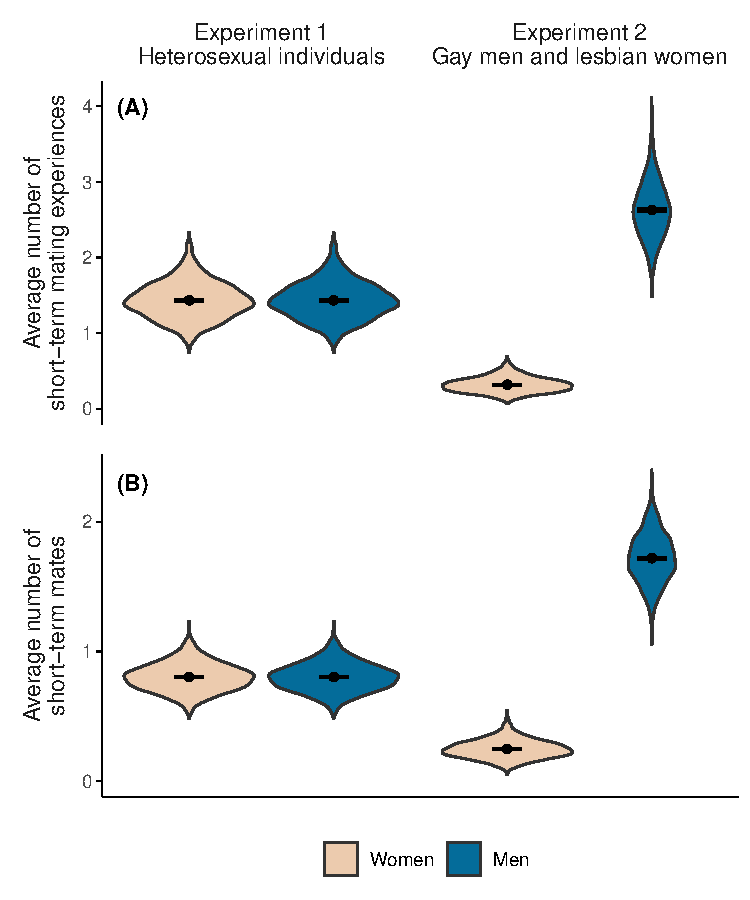
\includegraphics[width=100mm]{figures/fig1_men_vs_women.pdf}
  \caption{\textbf{Short-term mating behaviors of men and women after 1,000 time steps in the model when gender differences existed in mating preferences.} Violin plots summarizing the outcome variables separately for heterosexual individuals and gay men and lesbian women. Plot (A) shows the average number of short-term mating experiences, and plot (B) shows the average number of short-term mates. Central points show mean values and whiskers represent standard errors, but the standard errors are small and overlap to form a single bar. The averages were calculated using the full population of men and women in the model (\textit{N\textsubscript{men}} = \textit{N\textsubscript{women}} = 150).}
  \label{fig:men_vs_women}
\end{figure}

The results from Experiment 2 showed that when there were gender
differences in preferences for short-term mating, there were gender
differences in short-term mating behaviors between gay men and lesbian
women (Figure \ref{fig:men_vs_women}). The average number of short-term
mating experiences was higher among gay men (\emph{M} = 2.63, \emph{SD}
= 0.37) than among lesbian women (\emph{M} = 0.32, \emph{SD} = 0.10),
\emph{t}(4,998) = -301.78, \emph{p} \textless{} .001, Cohen's \emph{d} =
8.54. Similarly, the average number of short-term mates was higher among
gay men (\emph{M} = 1.72, \emph{SD} = 0.19) than among lesbian women
(\emph{M} = 0.25, \emph{SD} = 0.07), \emph{t}(4,998) = -357.69, \emph{p}
\textless{} .001, Cohen's \emph{d} = 10.12.

\hypertarget{heterosexual-individuals-in-the-mating-pool}{%
\subsection{Heterosexual individuals in the mating
pool}\label{heterosexual-individuals-in-the-mating-pool}}

In Experiment 1, there was a smaller proportion of heterosexual men in
the mating pool (\emph{M} = 0.38, \emph{SD} = 0.04) compared to women
(\emph{M} = 0.51, \emph{SD} = 0.05)), \emph{t}(4,998) = 104.85, \emph{p}
\textless{} .001, Cohen's \emph{d} = 2.97. In this population, there
were gender differences in short-term mating behaviors when men and
women had differential preferences for short-term mating (Figure
\textbf{x}). The average number of short-term mating experiences was
higher among heterosexual men (\emph{M} = 3.78, \emph{SD} = 0.50) than
among heterosexual women (\emph{M} = 2.79, \emph{SD} = 0.35),
\emph{t}(4,998) = -81.53, \emph{p} \textless{} .001, Cohen's \emph{d} =
2.31. Likewise, the average number of short-term mates was higher among
heterosexual men (\emph{M} = 2.12, \emph{SD} = 0.17) than among
heterosexual women (\emph{M} = 1.56, \emph{SD} = 0.11), \emph{t}(4,998)
= -135.85, \emph{p} \textless{} .001, Cohen's \emph{d} = 3.84.

\hypertarget{comparing-heterosexual-and-gay-men}{%
\subsection{Comparing heterosexual and gay
men}\label{comparing-heterosexual-and-gay-men}}

Gay men engaged in short-term mating behaviors more than heterosexual
men did (Figure \ref{fig:hetero_vs_gay}). The average number of
short-term mating experiences (as calculated using the full population
of men) was higher among gay men (\emph{M} = 2.63, \emph{SD} = 0.37)
than among heterosexual men (\emph{M} = 1.43, \emph{SD} = 0.24),
\emph{t}(4,998) = -134.87, \emph{p} \textless{} .001, Cohen's \emph{d} =
3.81. Similarly, the average number of short-term mates (as calculated
using the full population of men) was higher among gay men (\emph{M} =
1.72, \emph{SD} = 0.19) than among heterosexual men (\emph{M} = 0.80,
\emph{SD} = 0.11), \emph{t}(4,998) = -206.91, \emph{p} \textless{} .001,
Cohen's \emph{d} = 5.85.

\begin{figure}[h]
  \centering
  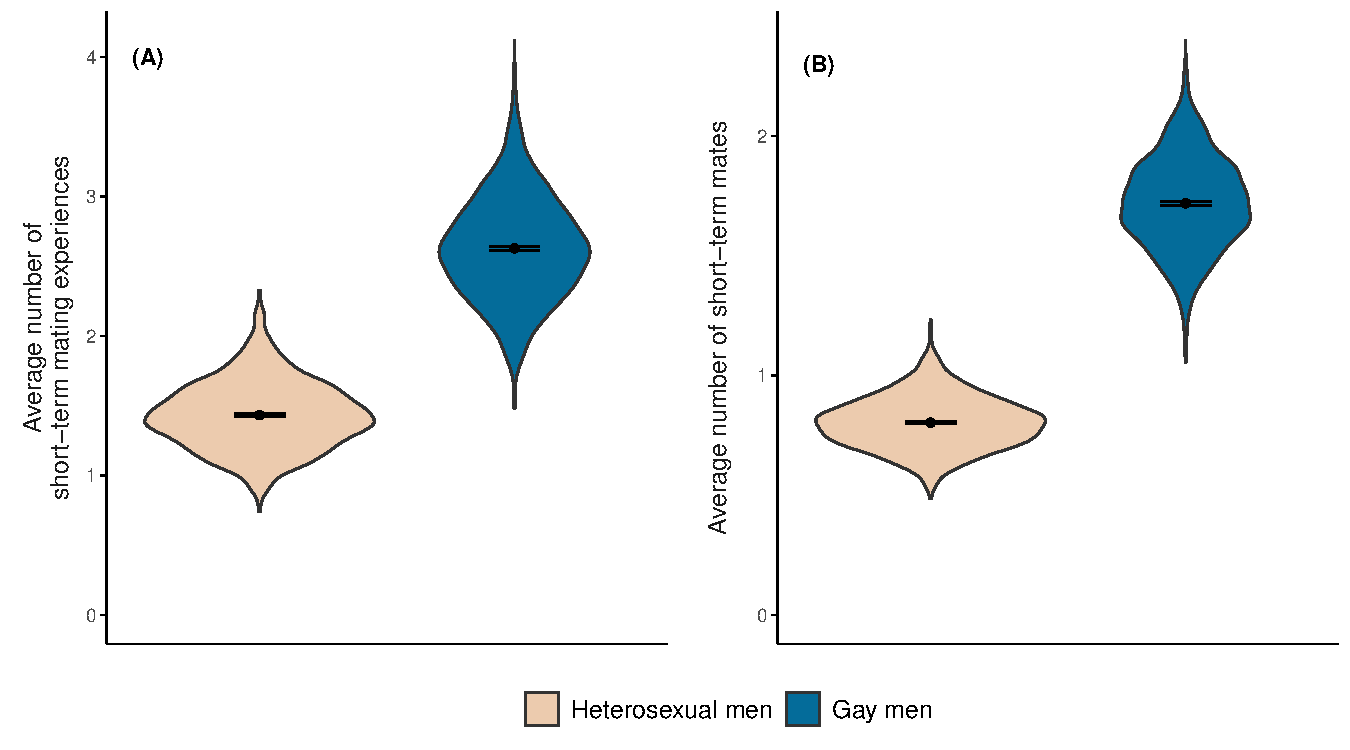
\includegraphics[width=0.8\columnwidth]{figures/fig3_hetero_vs_gay_men.pdf}
  \caption{\textbf{Short-term mating behaviors of heterosexual and gay men after 1,000 time steps in the model when gender differences existed in mating preferences.} Violin plots summarizing the outcome variables. Plot (A) shows the average number of short-term mating experiences, and plot (B) shows the average number of short-term mates. Central points show mean values and whiskers represent standard errors, but the standard errors are small and overlap to form a single bar. The averages were calculated using the full population of heterosexual and gay men in the model (\textit{N\textsubscript{hetero}} = \textit{N\textsubscript{gay}} = 150).}
  \label{fig:hetero_vs_gay}
\end{figure}

\hypertarget{comparing-across-conditions}{%
\subsection{Comparing across
conditions}\label{comparing-across-conditions}}

We also ran analyses across conditions to see which of the two
dimensions of mating preferences contributed to gender differences in
short-term mating behaviors.

Among heterosexual individuals, gender differences in short-term mating
behaviors, when calculated among individuals in the mating pool, emerged
when men and women had different standards for short-term mates.
Heterosexual men (vs.~heterosexual women) in the mating pool had a
higher average number of short-term mating experiences and short-term
mates as long as they had lower mating standards, even when no gender
difference existed in short-term mating likelihood (experiences:
\emph{M\textsubscript{men}} = 2.82, \emph{SD\textsubscript{men}} = 0.36,
\emph{M\textsubscript{women}} = 2.21, \emph{SD\textsubscript{women}} =
0.28, Cohen's \emph{d} = 1.89; partners: \emph{M\textsubscript{men}} =
1.76, \emph{SD\textsubscript{men}} = 0.15; \emph{M\textsubscript{women}}
= 1.38, \emph{SD\textsubscript{women}} = 0.09, Cohen's \emph{d} = 3.13).
In comparison, virtually no gender differences in short-term mating
behaviors existed when men and women had the same mating standards
(Table 1).

\begin{table}

\caption{\label{tab:table_1}\textbf{Short-term mating behaviors of heterosexual men and women in the mating pool after 1,000 time steps in the model}}
\centering
\begin{threeparttable}
\resizebox{\linewidth}{!}{
\begin{tabular}[t]{>{\raggedright\arraybackslash}p{2in}llllllllll}
\toprule
\multicolumn{1}{c}{ } & \multicolumn{5}{c}{\makecell[c]{Average short-term mating\\experiences (in-pool)}} & \multicolumn{5}{c}{\makecell[c]{Average short-term\\mates (in-pool)}} \\
\cmidrule(l{3pt}r{3pt}){2-6} \cmidrule(l{3pt}r{3pt}){7-11}
\multicolumn{1}{c}{ } & \multicolumn{2}{c}{Men} & \multicolumn{2}{c}{Women} & \multicolumn{1}{c}{ } & \multicolumn{2}{c}{Men} & \multicolumn{2}{c}{Women} & \multicolumn{1}{c}{ } \\
\cmidrule(l{3pt}r{3pt}){2-3} \cmidrule(l{3pt}r{3pt}){4-5} \cmidrule(l{3pt}r{3pt}){7-8} \cmidrule(l{3pt}r{3pt}){9-10}
\multicolumn{1}{c}{\em{ }} & \multicolumn{1}{c}{\em{M}} & \multicolumn{1}{c}{\em{SD}} & \multicolumn{1}{c}{\em{M}} & \multicolumn{1}{c}{\em{SD}} & \multicolumn{1}{c}{\em{d}} & \multicolumn{1}{c}{\em{M}} & \multicolumn{1}{c}{\em{SD}} & \multicolumn{1}{c}{\em{M}} & \multicolumn{1}{c}{\em{SD}} & \multicolumn{1}{c}{\em{d}}\\
\midrule
Same likelihood*Same standard & 2.21 & 0.38 & 2.20 & 0.37 & 0.03 & 1.39 & 0.12 & 1.39 & 0.12 & 0.04\\
Same likelihood*Different standard & 2.82 & 0.36 & 2.21 & 0.28 & 1.89 & 1.76 & 0.15 & 1.38 & 0.09 & 3.13\\
Different likelihood*Same standard & 2.80 & 0.48 & 2.78 & 0.47 & 0.03 & 1.57 & 0.14 & 1.56 & 0.14 & 0.05\\
Different likelihood*Different standard & 3.78 & 0.50 & 2.79 & 0.35 & 2.31 & 2.12 & 0.17 & 1.56 & 0.11 & 3.84\\
\bottomrule
\end{tabular}}
\begin{tablenotes}
\small
\item \textit{Note.} The averages were calculated with subsamples of men and women who had had engaged in short-term mating behaviors. See Supplementary Materials for the mean and standard deviation of sample sizes.
\end{tablenotes}
\end{threeparttable}
\end{table}

Among gay men and lesbian women, gender differences in short-term mating
behaviors emerged both when they had different short-term mating
likelihood and when their mating standards were different. Gay men
(vs.~lesbian women) had a higher average number of short-term mating
experiences and short-term mates when they had a higher short-term
mating likelihood (experiences: \emph{M\textsubscript{men}} = 0.80,
\emph{SD\textsubscript{men}} = 0.23, \emph{M\textsubscript{women}} =
0.32, \emph{SD\textsubscript{women}} = 0.10, Cohen's \emph{d} = 2.67;
partners: \emph{M\textsubscript{men}} = 0.52,
\emph{SD\textsubscript{men}} = 0.13, \emph{M\textsubscript{women}} =
0.25, \emph{SD\textsubscript{women}} = 0.07, Cohen's \emph{d} = 2.60),
or when they had lower mating standards (experiences:
\emph{M\textsubscript{men}} = 1.05, \emph{SD\textsubscript{men}} = 0.18,
\emph{M\textsubscript{women}} = 0.32, \emph{SD\textsubscript{women}} =
0.10, Cohen's \emph{d} = 5.10; partners: \emph{M\textsubscript{men}} =
0.82, \emph{SD\textsubscript{men}} = 0.12, \emph{M\textsubscript{women}}
= 0.25, \emph{SD\textsubscript{women}} = 0.07, Cohen's \emph{d} = 5.78).
In comparison, virtually no gender differences in short-term mating
behaviors existed when gay men and lesbian women had the same short-term
mating likelihood and mating standards (Table 2).

\begin{table}

\caption{\label{tab:table_2}\textbf{Short-term mating behaviors of gay men and lesbian women after 1,000 time steps in the model}}
\centering
\begin{threeparttable}
\resizebox{\linewidth}{!}{
\begin{tabular}[t]{>{\raggedright\arraybackslash}p{2in}llllllllll}
\toprule
\multicolumn{1}{c}{ } & \multicolumn{5}{c}{\makecell[c]{Average short-term mating\\experiences}} & \multicolumn{5}{c}{Average short-term mates} \\
\cmidrule(l{3pt}r{3pt}){2-6} \cmidrule(l{3pt}r{3pt}){7-11}
\multicolumn{1}{c}{ } & \multicolumn{2}{c}{Men} & \multicolumn{2}{c}{Women} & \multicolumn{1}{c}{ } & \multicolumn{2}{c}{Men} & \multicolumn{2}{c}{Women} & \multicolumn{1}{c}{ } \\
\cmidrule(l{3pt}r{3pt}){2-3} \cmidrule(l{3pt}r{3pt}){4-5} \cmidrule(l{3pt}r{3pt}){7-8} \cmidrule(l{3pt}r{3pt}){9-10}
\multicolumn{1}{c}{\em{ }} & \multicolumn{1}{c}{\em{M}} & \multicolumn{1}{c}{\em{SD}} & \multicolumn{1}{c}{\em{M}} & \multicolumn{1}{c}{\em{SD}} & \multicolumn{1}{c}{\em{d}} & \multicolumn{1}{c}{\em{M}} & \multicolumn{1}{c}{\em{SD}} & \multicolumn{1}{c}{\em{M}} & \multicolumn{1}{c}{\em{SD}} & \multicolumn{1}{c}{\em{d}}\\
\midrule
Same likelihood*Same standard & 0.32 & 0.10 & 0.32 & 0.10 & 0.04 & 0.25 & 0.07 & 0.25 & 0.07 & 0.03\\
Same likelihood*Different standard & 1.05 & 0.18 & 0.32 & 0.10 & 5.10 & 0.82 & 0.12 & 0.25 & 0.07 & 5.78\\
Different likelihood*Same standard & 0.80 & 0.23 & 0.32 & 0.10 & 2.67 & 0.52 & 0.13 & 0.25 & 0.07 & 2.60\\
Different likelihood*Different standard & 2.63 & 0.37 & 0.32 & 0.10 & 8.54 & 1.72 & 0.19 & 0.25 & 0.07 & 10.12\\
\bottomrule
\end{tabular}}
\begin{tablenotes}
\small
\item \textit{Note.} \textit{N\textsubscript{men}} = \textit{N\textsubscript{women}} = 150 in all conditions.
\end{tablenotes}
\end{threeparttable}
\end{table}

\hypertarget{discussion}{%
\section{Discussion}\label{discussion}}

The present study used agent-based modeling to investigate whether men
and women's differential preferences for short-term mating would result
in gender differences in short-term mating behaviors, and if so, then
under what conditions they would result in differences in the number of
short-term mating experiences and short-term mates. We formulated two
hypotheses: 1) gay men would engage in more short-term mating behaviors
as compared to lesbian women, and 2) gay men would engage in more
short-term mating behaviors as compared to heterosexual men. The results
from 1,000 time steps in a model simulating men and women's mating
behaviors provided strong evidence in favor of our hypotheses. First of
all, as compared to lesbian women, gay men had higher average numbers of
short-term mating experiences and short-term mates. Secondly, gay men
also had higher average numbers of short-term mating experiences and
short-term mates as compared to heterosexual men. In contrast, we found
no gender differences in short-term mating behaviors between
heterosexual men and women, although heterosexual men in the mating pool
had higher average numbers of short-term mating experiences and
short-term mates.

As expected, heterosexual men and women did not differ in short-term
mating behaviors despite their differential preferences for short-term
mating. This was because heterosexual men and women had an equal total
number of both short-term mating experiences and short-term mates. This
is not surprising since the sex ratio was 1:1 in our model. It therefore
follows that the average number of short-term mating experiences and
short-term mates must be equal between men and women as well. However,
we did find that when we only looked at individuals in the mating pool
(from which more men than women were excluded), men engaged in more
short-term mating behaviors as compared to women. This was because there
were more women than men in the mating pool, resulting in lower averages
among heterosexual women despite the equal numbers of experiences and
mates in total.

Moreover, gender differences in short-term mating behaviors emerged when
heterosexual men and women had different mating standards, but not when
they had different short-term mating likelihood. When women had a higher
standard than men did, less men than women in the population were above
a potential partner's standard and thus had a chance to have sex with
them. This contributed to the unequal number of men and women in the
mating pool, which led to gender differences in short-term mating
behaviors among this population. In comparison, even when men and women
had different short-term mating likelihood, the probability of any pair
of them ending up having sex is the product of their individual
likelihood (since men and women made decisions independently). As this
probability is the same for both parties, the gender difference in
short-term mating likelihood did not translate into different behaviors.

In the light of these results, previous empirical observations of gender
differences in short-term mating behaviors among heterosexual
individuals (e.g., Petersen \& Hyde, 2010) appear perplexing (e.g.,
Gurman, 1989). Possible explanations for these empirical results that
seem illogical considering the simulation findings may have to do with
features of the observation process. One possibility is sampling bias in
the observations (e.g., Wiederman \& Dubois, 1998) since surveys
regarding short-term mating behaviors may tend to attract individuals
who already engage in such behaviors. Our results suggest that when this
group of individuals is considered, there can be gender differences in
short-term mating behaviors that do not exist in the full population. A
second explanation is that heterosexual men and women's self-reported
sexual behaviors are affected by social desirability bias due to gender
norms. Men may overreport since having more sexual partners can show
their masculinity and yield them reputation benefits, while women may
underreport because this violates the chastity norm (Fisher, 2013). A
third explanation is that men and women have different estimation
strategies of their sexual experiences. Men may tend to approximate and
round up, while women's tendency to count instances may lead to lower
estimations (Brown \& Sinclair, 1999; Mitchell et al., 2019).

Among gay men and lesbian women, large gender differences in short-term
mating behaviors existed when men and women had differential preferences
for short-term mating, which was in line with empirical observations
(e.g., Peplau et al., 1997, 2004). This was likely because the number of
short-term mating experiences and short-term mates no longer counted
towards men and women simultaneously. Any gender differences in mating
preferences would result in differences in behaviors. A closer look at
the results did support this postulation. Both a difference in the
likelihood of short-term mating and in mating standards alone resulted
in gender differences in mating behaviors. This was likely because the
former increased the probability of both parties of a given gay couple
deciding to have short-term mating, and the latter increased the
probability of both meeting each other's standards, as compared to the
case of a given lesbian couple.

Also, as gay men's preferences for short-term mating were not
constrained by those of women, we found that gay men engaged in more
short-term mating behaviors compared to heterosexual men. This was
consistent with the empirical literature (e.g., Peplau et al., 1997).
Interestingly, gay men and heterosexual men had the same short-term
mating likelihood and the same standards for short-term mates in our
model. The only difference was a change in the preferences of potential
partners. When men's partners had a stronger preferences for short-term
mating (i.e., having men vs.~having women as potential partners), men
also appeared to engage in more short-term mating behaviors.

\hypertarget{conclusion}{%
\section{Conclusion}\label{conclusion}}

Using agent-based modeling to simulate short-term mating behaviors, we
found when men (vs.~women) had a stronger preferences for short-term
mating, heterosexual men and women engaged in short-term mating
behaviors to the same extent, while gay men engaged in more short-term
mating behaviors as compared to lesbian women. Gay men engaged in more
short-term mating behaviors than heterosexual men did.

These results highlight the distinction between preferences and
behaviors in human mating. Individuals' mating behaviors do not only
depend on one's own preferences, but are also constrained by partners'
preferences. Future research in human mating should not only focus on
the psychological aspect but also pay attention to the interaction
between individuals' psychology and its context. These results also cast
doubt to the prevalent belief in the gender differences in short-term
mating behaviors, especially among heterosexual individuals. Our
findings suggest that there may be factors in the observation process,
such as sampling bias, that contribute to the observed differences.
Future research in human sexuality should note such possibilities and
interpret any observed gender differences in short-term mating behaviors
cautiously.

\hypertarget{acknowledgements}{%
\section{Acknowledgements}\label{acknowledgements}}

\hypertarget{data-availability}{%
\section{Data availability}\label{data-availability}}

All models, data, and analysis code can be downloaded at: {[}link masked
for peer review{]}

\newpage

\hypertarget{references}{%
\section*{References}\label{references}}
\addcontentsline{toc}{section}{References}

\hypertarget{refs}{}
\begin{CSLReferences}{1}{0}
\leavevmode\vadjust pre{\hypertarget{ref-archer_reality_2019}{}}%
Archer, J. (2019). The reality and evolutionary significance of human
psychological sex differences. \emph{Biological Reviews}, \emph{94}(4),
1381--1415. \url{https://doi.org/10.1111/brv.12507}

\leavevmode\vadjust pre{\hypertarget{ref-bailey_effects_1994}{}}%
Bailey, J. M., Gaulin, S., Agyei, Y., \& Gladue, B. A. (1994). Effects
of gender and sexual orientation on evolutionarily relevant aspects of
human mating psychology. \emph{Journal of Personality and Social
Psychology}, \emph{66}(6), 1081--1093.
\url{https://doi.org/10.1037/0022-3514.66.6.1081}

\leavevmode\vadjust pre{\hypertarget{ref-brown_estimating_1999}{}}%
Brown, N. R., \& Sinclair, R. C. (1999). Estimating number of lifetime
sexual partners: Men and women do it differently. \emph{The Journal of
Sex Research}, \emph{36}(3), 292--297.
\url{https://doi.org/10.1080/00224499909551999}

\leavevmode\vadjust pre{\hypertarget{ref-bryant_relationship_1994}{}}%
Bryant, A. S., \& Demian. (1994). Relationship characteristics of
american gay and lesbian couples. \emph{Journal of Gay \& Lesbian Social
Services}, \emph{1}(2), 101--117.
\url{https://doi.org/10.1300/J041v01n02_06}

\leavevmode\vadjust pre{\hypertarget{ref-buss_sexual_1993}{}}%
Buss, D. M., \& Schmitt, D. P. (1993). Sexual strategies theory: An
evolutionary perspective on human mating. \emph{Psychological Review},
\emph{100}(2), 204--232.
\url{https://doi.org/doi:10.1037/0033-295X.100.2.204d}

\leavevmode\vadjust pre{\hypertarget{ref-buss2019mate}{}}%
Buss, D. M., \& Schmitt, D. P. (2019). Mate preferences and their
behavioral manifestations. \emph{Annual Review of Psychology},
\emph{70}, 77--110.

\leavevmode\vadjust pre{\hypertarget{ref-conley_women_2011}{}}%
Conley, T. D., Moors, A. C., Matsick, J. L., Ziegler, A., \& Valentine,
B. A. (2011). Women, men, and the bedroom: Methodological and conceptual
insights that narrow, reframe, and eliminate gender differences in
sexuality. \emph{Current Directions in Psychological Science},
\emph{20}(5), 296--300. \url{https://doi.org/10.1177/0963721411418467}

\leavevmode\vadjust pre{\hypertarget{ref-fisher2013gender}{}}%
Fisher, T. D. (2013). Gender roles and pressure to be truthful: The
bogus pipeline modifies gender differences in sexual but not non-sexual
behavior. \emph{Sex Roles}, \emph{68}(7), 401--414.

\leavevmode\vadjust pre{\hypertarget{ref-s_j_gurman_six_1989}{}}%
Gurman, S. J. (1989). Six of one... \emph{Nature}, \emph{12}, 342.
\url{https://www.nature.com/articles/342012d0}

\leavevmode\vadjust pre{\hypertarget{ref-hald_receptivity_2010}{}}%
Hald, G. M., \& Høgh-Olesen, H. (2010). Receptivity to sexual
invitations from strangers of the opposite gender. \emph{Evolution and
Human Behavior}, \emph{31}(6), 453--458.
\url{https://doi.org/10.1016/j.evolhumbehav.2010.07.004}

\leavevmode\vadjust pre{\hypertarget{ref-herbenick_sexual_2017}{}}%
Herbenick, D., Bowling, J., Fu, T.-C. (Jane)., Dodge, B., Guerra-Reyes,
L., \& Sanders, S. (2017). Sexual diversity in the {United States}:
Results from a nationally representative probability sample of adult
women and men. \emph{{PLOS} {ONE}}, \emph{12}(7), e0181198.
\url{https://doi.org/10.1371/journal.pone.0181198}

\leavevmode\vadjust pre{\hypertarget{ref-kenrick_evolution_1990}{}}%
Kenrick, D. T., Sadalla, E. K., Groth, G., \& Trost, M. R. (1990).
Evolution, traits, and the stages of human courtship: Qualifying the
parental investment model. \emph{Journal of Personality}, \emph{58}(1),
97--116. \url{https://doi.org/10.1111/j.1467-6494.1990.tb00909.x}

\leavevmode\vadjust pre{\hypertarget{ref-matsick_gender_2021}{}}%
Matsick, J. L., Kruk, M., Conley, T. D., Moors, A. C., \& Ziegler, A.
(2021). Gender similarities and differences in casual sex acceptance
among lesbian women and gay men. \emph{Archives of Sexual Behavior},
\emph{50}(3), 1151--1166.
\url{https://doi.org/10.1007/s10508-020-01864-y}

\leavevmode\vadjust pre{\hypertarget{ref-mcburney_preferred_2005}{}}%
McBurney, D. H., Zapp, D. J., \& Streeter, S. A. (2005). Preferred
number of sexual partners: Tails of distributions and tales of mating
systems. \emph{Evolution and Human Behavior}, \emph{26}(3), 271--278.
\url{https://doi.org/10.1016/j.evolhumbehav.2004.09.005}

\leavevmode\vadjust pre{\hypertarget{ref-mitchell_why_2019}{}}%
Mitchell, K. R., Mercer, C. H., Prah, P., Clifton, S., Tanton, C.,
Wellings, K., \& Copas, A. (2019). Why do men report more opposite-sex
sexual partners than women? Analysis of the gender discrepancy in a
british national probability survey. \emph{The Journal of Sex Research},
\emph{56}(1), 1--8. \url{https://doi.org/10.1080/00224499.2018.1481193}

\leavevmode\vadjust pre{\hypertarget{ref-oliver_gender_1993}{}}%
Oliver, M. B., \& Hyde, J. S. (1993). Gender differences in sexuality: A
meta-analysis. \emph{Psychological Bulletin}, \emph{114}(1), 29--51.
https://doi.org/\url{http://dx.doi.org/10.1037/0033-2909.114.1.29}

\leavevmode\vadjust pre{\hypertarget{ref-peplau_national_1997}{}}%
Peplau, L. A., Cochran, S. D., \& Mays, V. (1997). A national survey of
the intimate relationships of african american lesbians and gay men: A
look at commitment, satisfaction, sexual behavior, and {HIV} disease. In
\emph{Ethnic and cultural diversity among lesbians and gay men} (pp.
11--38). Sage Publications.

\leavevmode\vadjust pre{\hypertarget{ref-peplau_sexuality_2004}{}}%
Peplau, L. A., Fingerhut, A., \& Beals, K. P. (2004). Sexuality in the
relationships of lesbians and gay men. In \emph{The handbook of
sexuality in close relationships} (pp. 349--369). Lawrence Erlbaum
Associates Publishers.

\leavevmode\vadjust pre{\hypertarget{ref-petersen_meta-analytic_2010}{}}%
Petersen, J. L., \& Hyde, J. S. (2010). A meta-analytic review of
research on gender differences in sexuality, 1993--2007.
\emph{Psychological Bulletin}, \emph{136}(1), 21--38.
\url{https://doi.org/10.1037/a0017504}

\leavevmode\vadjust pre{\hypertarget{ref-r}{}}%
R Core Team. (2022). \emph{R: A language and environment for statistical
computing}. R Foundation for Statistical Computing.
\url{https://www.R-project.org/}

\leavevmode\vadjust pre{\hypertarget{ref-regan_minimum_1998}{}}%
Regan, P. C. (1998). Minimum mate selection standards as a function of
perceived mate value, relationship context, and gender. \emph{Journal of
Psychology \& Human Sexuality}, \emph{10}(1), 53--73.
\url{https://doi.org/10.1300/J056v10n01_04}

\leavevmode\vadjust pre{\hypertarget{ref-rissel_heterosexual_2014}{}}%
Rissel, C., Badcock, P. B., Smith, A. M. A., Richters, J., Visser, R. O.
de, Grulich, A. E., Simpson, J. M., Rissel, C., Badcock, P. B., Smith,
A. M. A., Richters, J., Visser, R. O. de, Grulich, A. E., \& Simpson, J.
M. (2014). Heterosexual experience and recent heterosexual encounters
among {A}ustralian adults: The second {A}ustralian study of health and
relationships. \emph{Sexual Health}, \emph{11}(5), 416--426.
\url{https://doi.org/10.1071/SH14105}

\leavevmode\vadjust pre{\hypertarget{ref-schmitt_universal_2003}{}}%
Schmitt, D. P. (2003). Universal sex differences in the desire for
sexual variety: Tests from 52 nations, 6 continents, and 13 islands.
\emph{Journal of Personality and Social Psychology}, \emph{85}(1), 85.
\url{https://doi.org/10.1037/0022-3514.85.1.85}

\leavevmode\vadjust pre{\hypertarget{ref-schmitt_are_2001}{}}%
Schmitt, D. P., Shackelford, T. K., \& Buss, D. M. (2001). Are men
really more 'oriented' toward short-term mating than women? A critical
review of theory and research. \emph{Psychology, Evolution \& Gender},
\emph{3}(3), 211--239. \url{https://doi.org/10.1080/14616660110119331}

\leavevmode\vadjust pre{\hypertarget{ref-symons_evolution_1979}{}}%
Symons, D. (1979). \emph{The evolution of human sexuality}. Oxford
University Press.

\leavevmode\vadjust pre{\hypertarget{ref-walter_sex_2020}{}}%
Walter, K. V., Conroy-Beam, D., Buss, D. M., Asao, K., Sorokowska, A.,
Sorokowski, P., Aavik, T., Akello, G., Alhabahba, M. M., Alm, C., Amjad,
N., Anjum, A., Atama, C. S., Atamtürk Duyar, D., Ayebare, R., Batres,
C., Bendixen, M., Bensafia, A., Bizumic, B., \ldots{} Zupančič, M.
(2020). Sex differences in mate preferences across 45 countries: A
large-scale replication. \emph{Psychological Science}, \emph{31}(4),
408--423. \url{https://doi.org/10.1177/0956797620904154}

\leavevmode\vadjust pre{\hypertarget{ref-ggplot2}{}}%
Wickham, H. (2016). \emph{{ggplot2: Elegant Graphics for Data
Analysis}}. Springer-Verlag New York.
\url{https://ggplot2.tidyverse.org}

\leavevmode\vadjust pre{\hypertarget{ref-wiederman_evolution_1998}{}}%
Wiederman, M. W., \& Dubois, S. L. (1998). Evolution and sex differences
in preferences for short-term mates: Results from a policy capturing
study. \emph{Evolution and Human Behavior}, \emph{19}(3), 153--170.
\url{https://doi.org/10.1016/S1090-5138(98)00006-3}

\leavevmode\vadjust pre{\hypertarget{ref-wilensky_1999}{}}%
Wilensky, U. (1999). \emph{NetLogo}
{[}Http://ccl.northwestern.edu/netlogo/{]}. Center for Connected
Learning; Computer-Based Modeling.
\url{http://ccl.northwestern.edu/netlogo/}

\end{CSLReferences}

\end{document}
